\begin{figure}[!b]
    \centering
    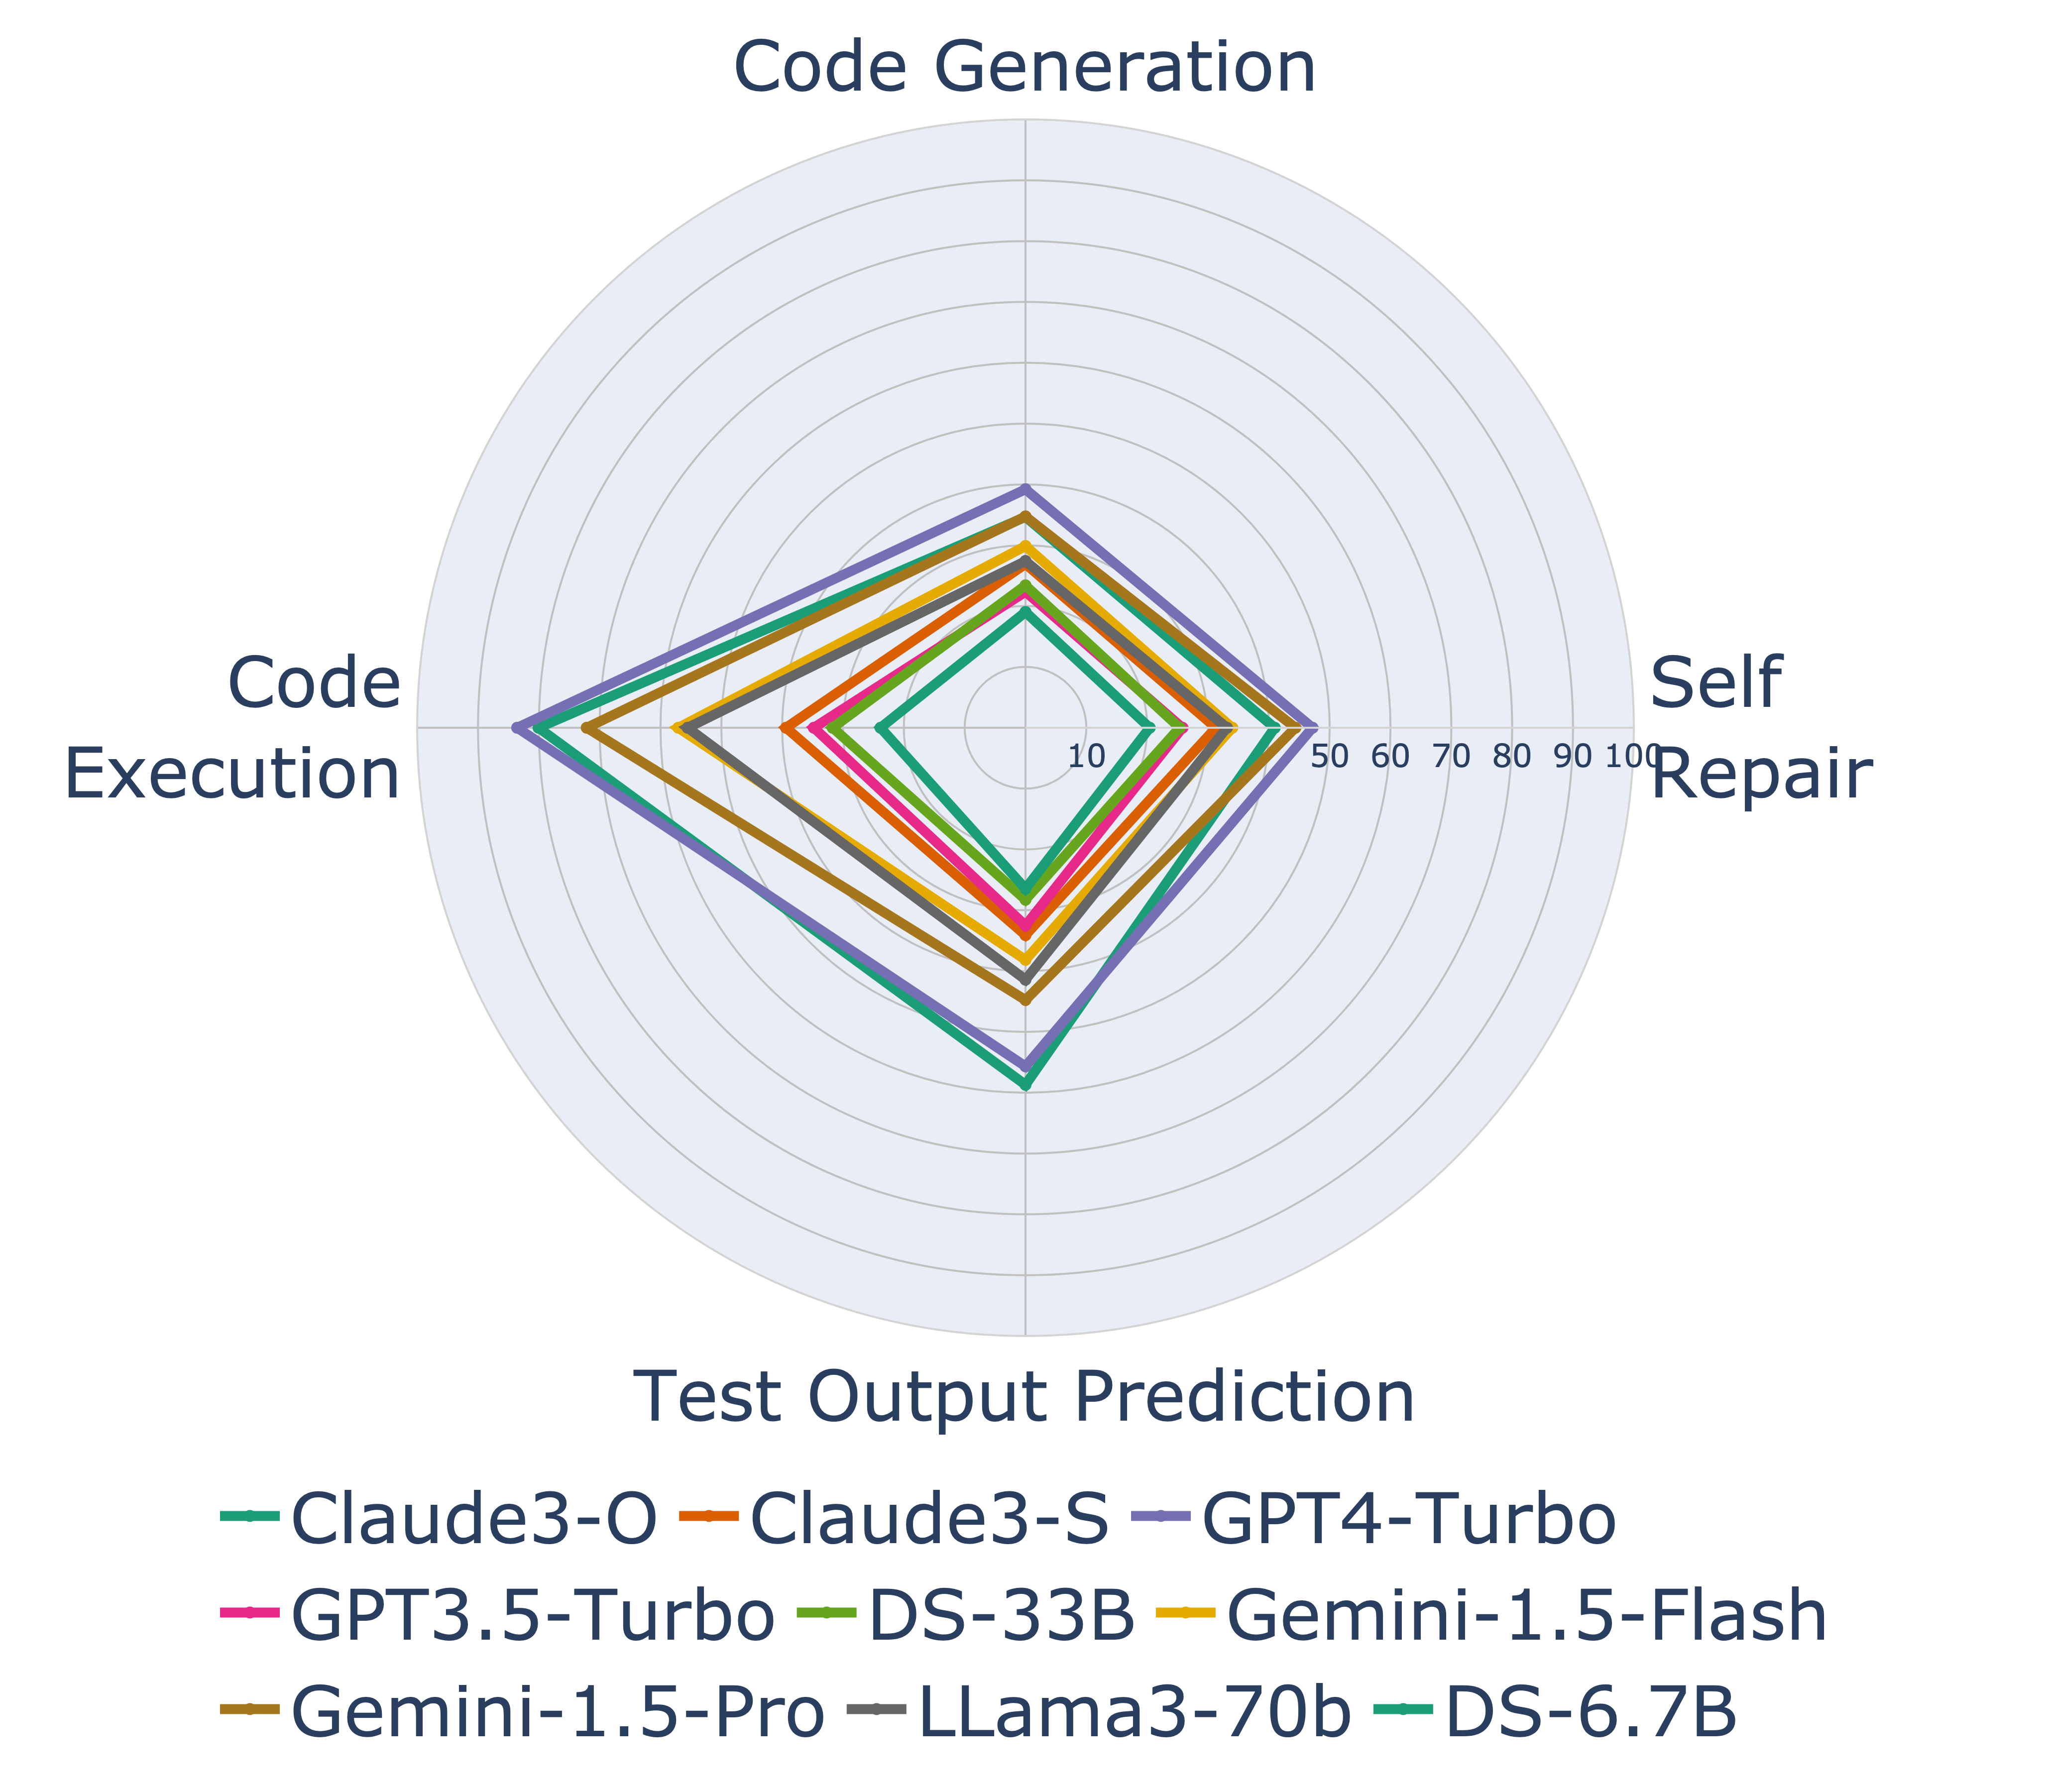
\includegraphics[width=0.47\linewidth]{figures/overview/tasks_radar.png}
    \hfil%
    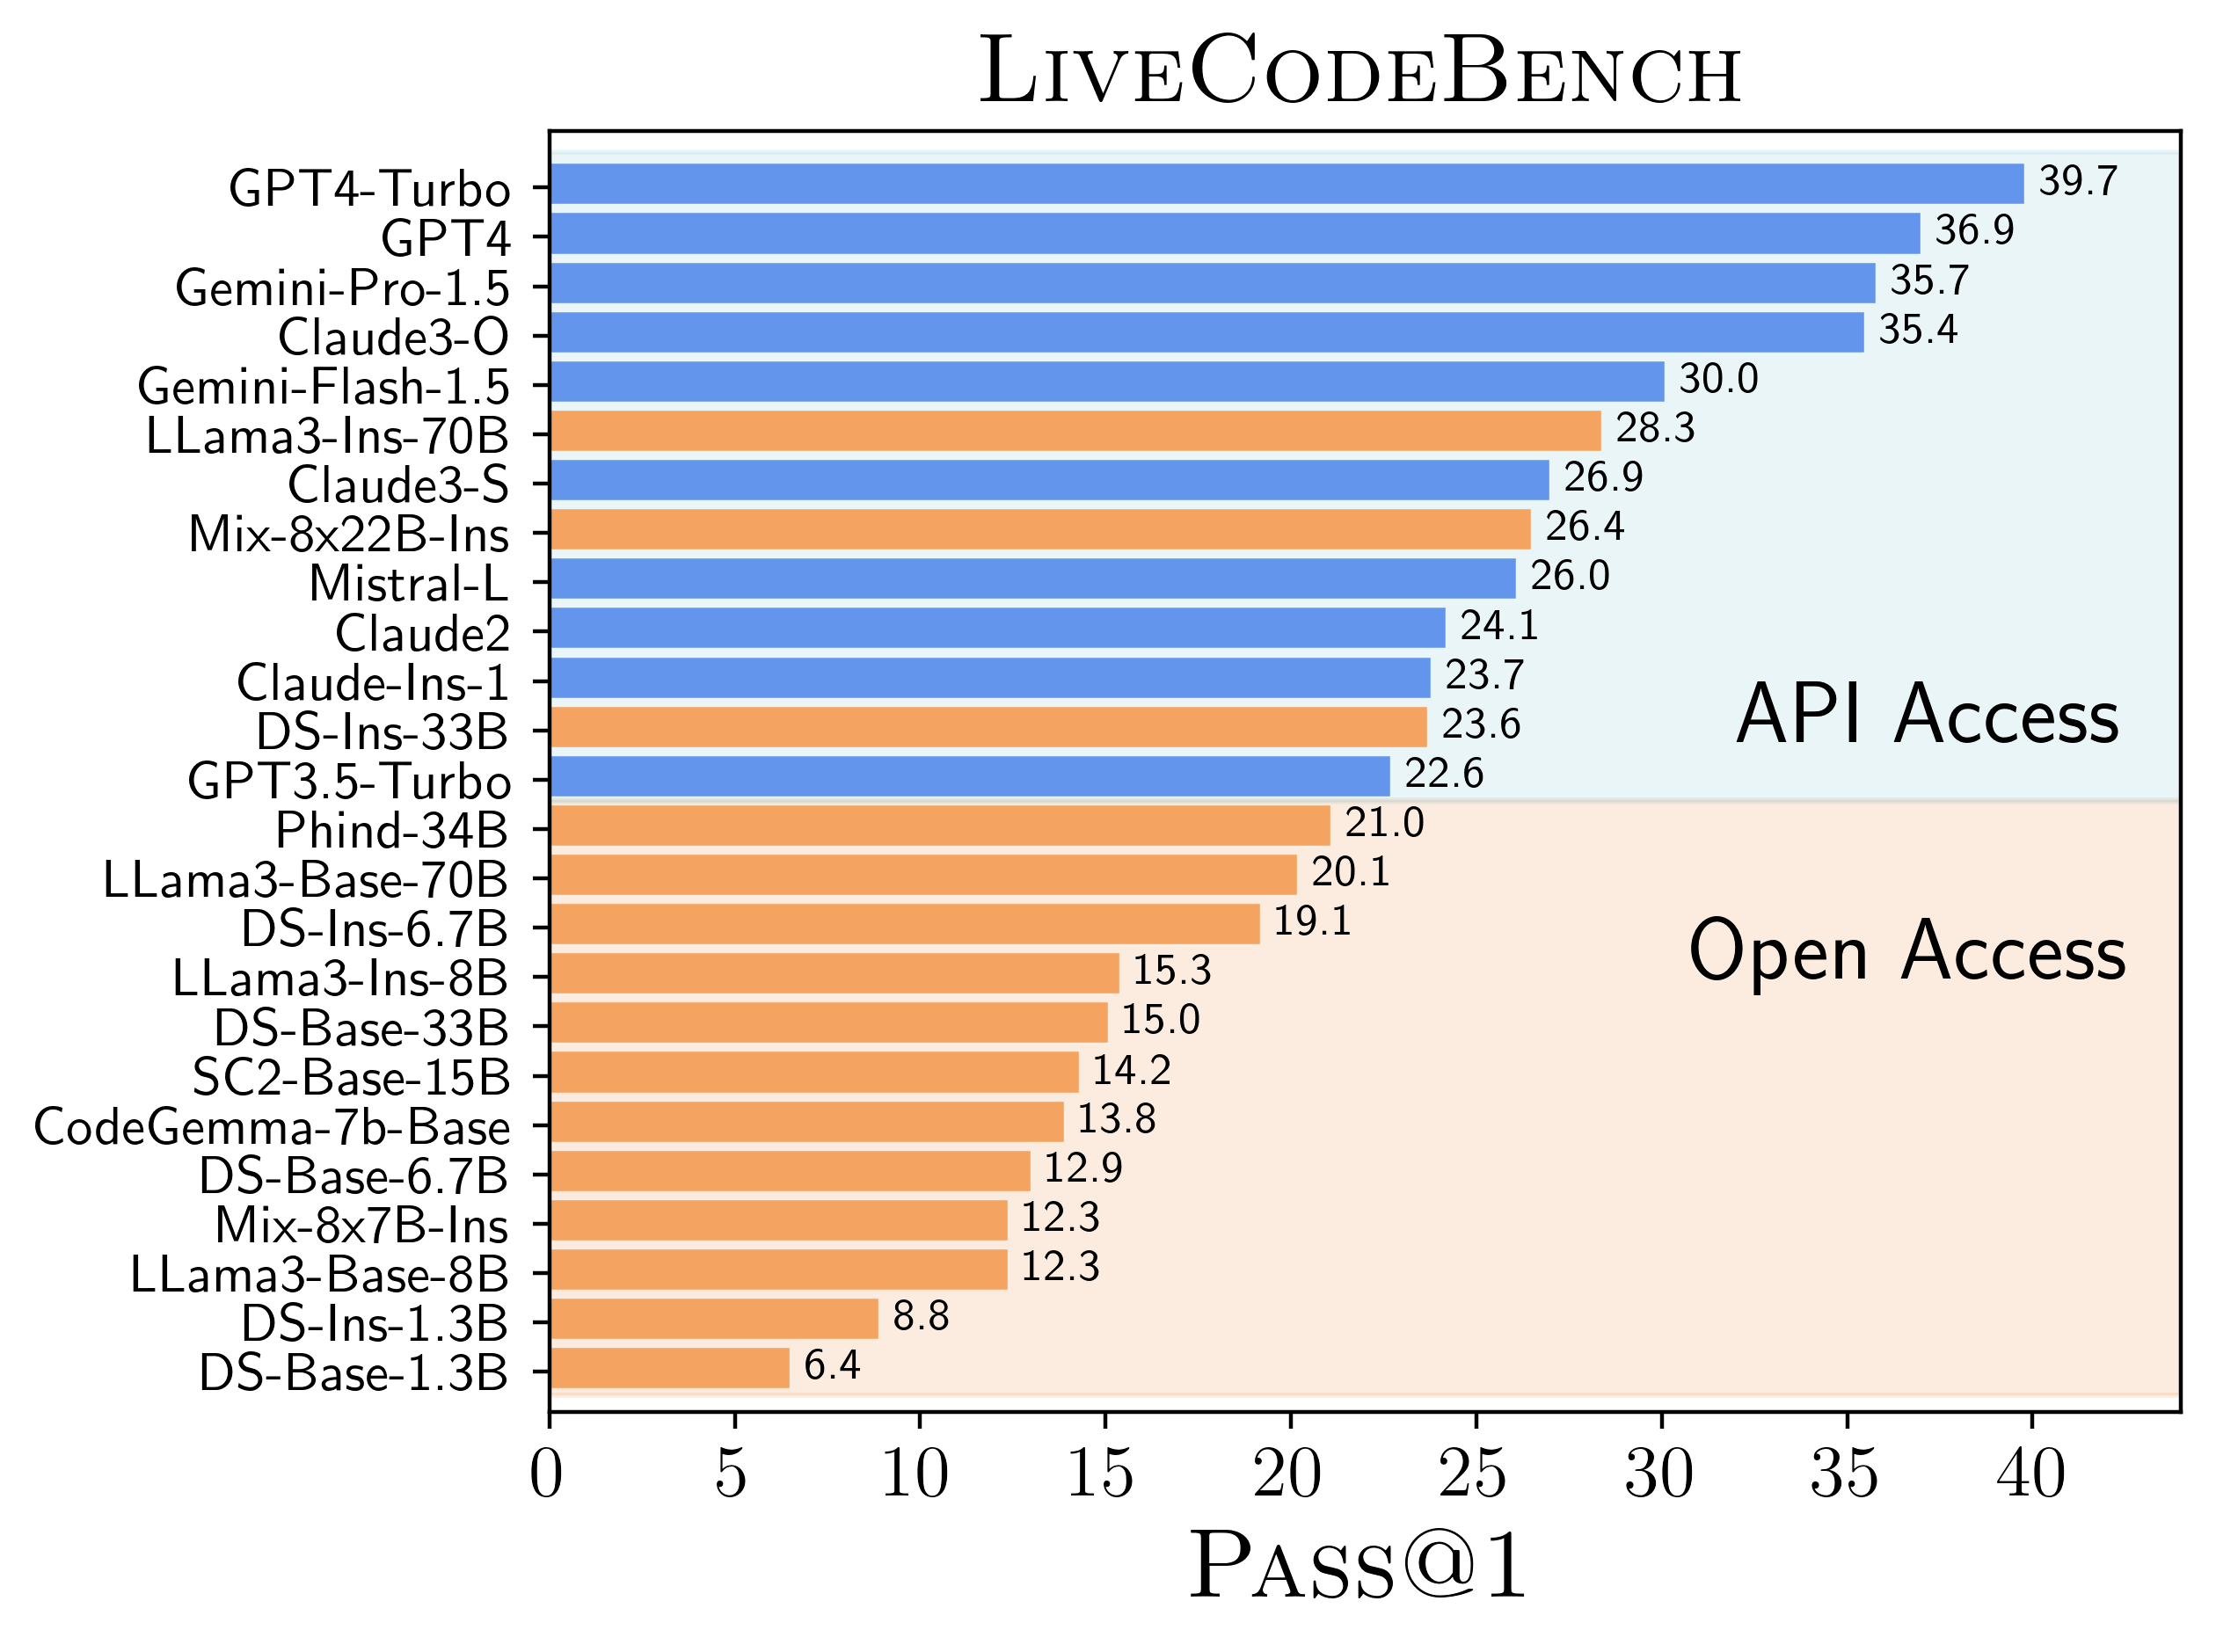
\includegraphics[width=0.52\linewidth]{figures/overview/lc_barchart.png}%
    % 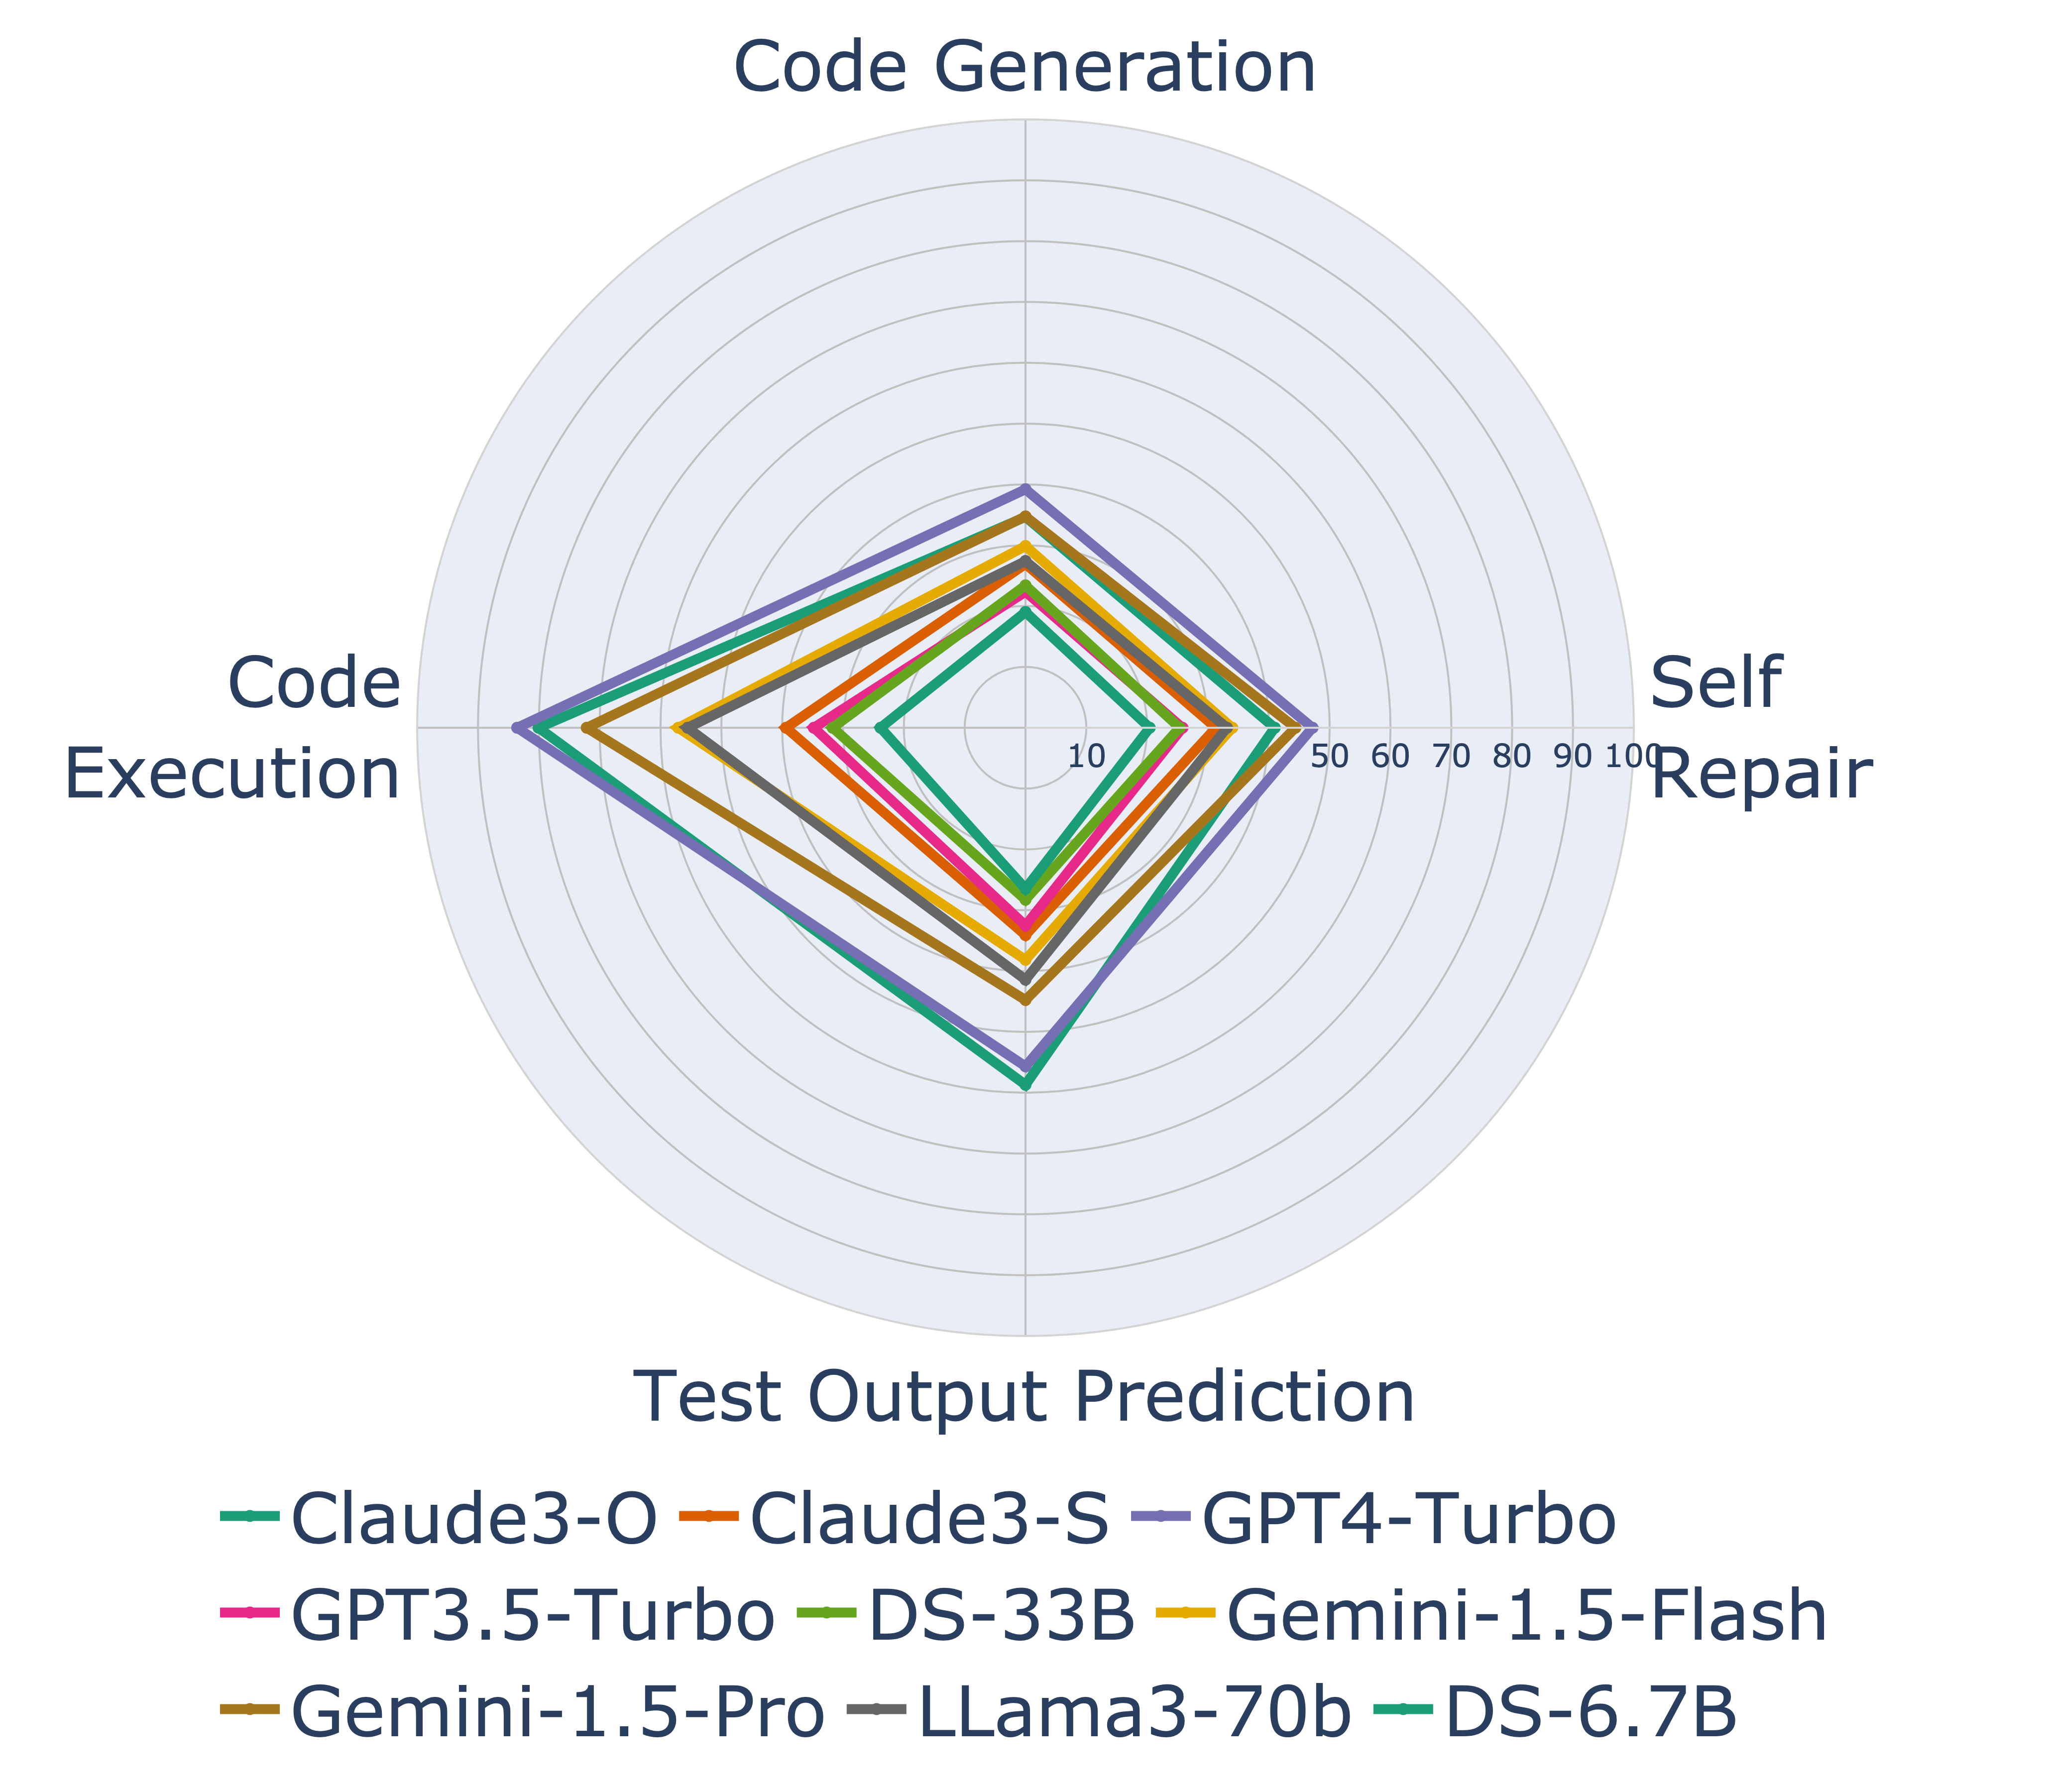
\includegraphics[width=0.5\textwidth]{figures/overview/tasks_radar.png}
    \caption{
        \textbf{Left.} 
        %\ag{maybe make axis 0 to 70 so it doesn't look like test output prediction gets perfect score. also axis labels could be bigger?}
        We propose evaluating \llms{} across 
        scenarios capturing various coding-related capabilities.
        Specifically, we host four different scenarios, namely code generation, 
        self-repair, code execution, and test output prediction.
        The figure depicts various model performances across the four scenarios available in \livecodebench{} in a radial plot -- 
        highlighting how relative differences across models change across the scenarios.
        \textbf{Right.}
        Comparison of open access and (closed) API access models on \livecodebench{}-Easy 
        code generation scenario. We find that closed-access models consistently 
        outperform the open models with only strong instruction-tuned variants of $>30$\textsc{B}
        models (specifically \llamaB{70}, \mixtral and  \deepseekcodeB{33} models) crossing the performance gap.
        }
    \label{fig:all_tasks_radial}
\end{figure}
